%Funktion

\ihead{\headmark}
\ohead{Lars Strölin, Michael Geigges, Ilja Kononenko}
\automark{section}
\cfoot{\pagemark}


\section{Funktion}

\textbf{Funktionen und Aufbau im Überblick:}

\begin{enumerate}[label=\Roman*)]
	\item Eingabe
	\item Zeichnen
	\item Berechnen
	\item Hilfe
\end{enumerate}

%-----------------------------------------------------------------------------------------

\subsection{Eingabe}
Um eine Funktion eingeben zu können verwendet man das erste Eingabefeld links oben neben der Beschriftung "Funktion: ". Dort kann man dann eine X-beliebige Funktion eingeben, welche später auf dem KOS angezeigt werden kann.
\newline
Für die Berechnung eines Y-Wertes gibt es das zweite Eingabefeld rechts daneben mit der Beschriftung "X-Wert: ". Hier kann auch einen komplett beliebigen Wert mit einem "X" eingeben.

\begin{figure}[ht]
	\centering
	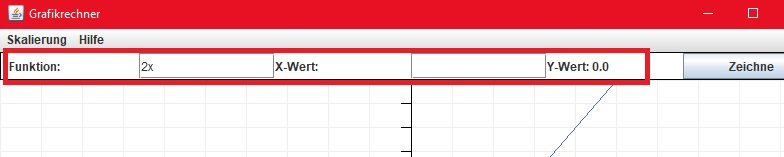
\includegraphics[width=1.0\textwidth]{Bilder/GR_2.jpg}
	\caption{Erstes und zweites Eingabefeld}
\end{figure}

%-----------------------------------------------------------------------------------------

\subsection{Zeichnen}
Um die Funktion dann auf dem Koordinatensystem anzeigen zu lassen benutzt man rechts oben im Eck den "Zeichne"-Button. Danach wird in anderer Farbe sofort auf dem Feld die Funktion gezeichnet und und korrekt angezeigt.

\begin{figure}[ht]
	\centering
	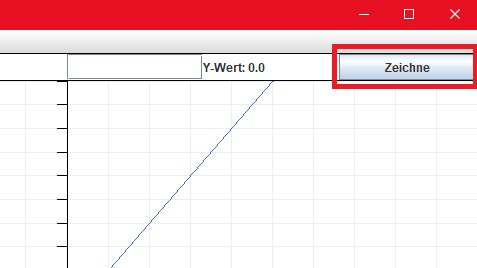
\includegraphics[width=0.6\textwidth]{Bilder/GR_3.jpg}
	\caption{Zeichne-Button}
\end{figure}


\subsubsection{Skalierung}
Die standardmäßige Größe des KOS (Koordinatensystem) beträgt in alle vier Richtungen 10 bzw. -10.
Aufgrund dessen, dass gewisse Funktionen ihre wichtigen Punkte in darüber liegenden Werten besitzen, oder der Benutzer einfach einen anderen Bereich gerne anschauen will, gibt es eine Einstellung für die Skalierung. 
\newline
In der Menüleiste gibt es links oben als erster Punkt das Menüitem Skalierung. Drückt man auf diesen Punkt öffnet sich ein Unterpunkt und unter dort kann man dann über ein Fenster, welches sich dann extra öffnet, die vier Werte der Skalierung manuell seinen Wünschen anpassen. Über den Punkt "Skalierung einstellen" werden die Werte auf der Anzeige übernommen. Der Punkt "Standard Skalierung" stellt die üblichen Werte 10 bzw. -10 wieder her.

\begin{figure}[ht]
	\begin{center}
		\subfloat[Menüitem Skalierung]{
		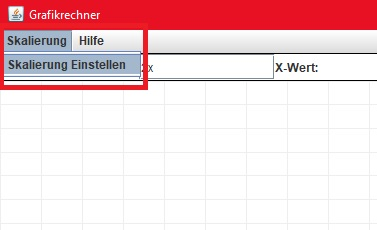
\includegraphics[width=0.4\textwidth]{Bilder/GR_4.jpg} }
	\hspace{1cm}
		\subfloat[Einstellungen für die Skalierung]{
		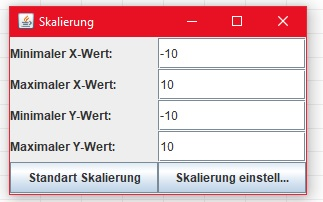
\includegraphics[width=0.4\textwidth]{Bilder/GR_5.jpg} }
	\end{center}
\end{figure}

%-----------------------------------------------------------------------------------------

\subsection{Berechnen}
Nach Eingabe einer Funktion im zweiten Eingabefeld gibt es rechts oben speziell für den Y-Wert ein Ausgabefeld. Um den Y-Wert zu erhalten muss man lediglich nach der Eingabe die "ENTER"-Taste drücken.

\subsubsection{Besondere Werte} 
In der Mathematik gibt es bestimmte Werte die von besonderer Bedeutung sind, wie z.B die Nullstellen, Hoch- und Tiefpunkte (Extrempunkte) oder die Ableitung. Auch dafür bietet das Programm unter dem KOS eine Lösung. Hier befinden sich jeweils drei Ausgabefelder mit einem "Berechne"-Button. Wird dieser nach einer korrekten Eingabe im ersten Eingabefeld gedrückt, werden die jeweiligen Werte berechnet und ausgegeben.

\begin{figure}[ht]
	\centering
	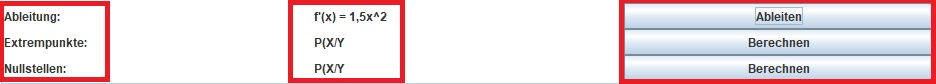
\includegraphics[width=1.0\textwidth]{Bilder/GR_6.jpg}
	\caption{Ausgabefelder für besondere Werte}
\end{figure}

\newpage

%-----------------------------------------------------------------------------------------

\subsection{Hilfe}
In der Menüleiste gibt es neben der Skalierung noch den zweiten Punkt "Hilfe". Dort kommt man zu den Unterpunkten "Anleitung" und "Über". 
\newline
Bei der Anleitung öffnet sich auch ein extra Fenster mit einer kleinen Anleitung um die Hauptfunktionen noch einmal zu erklären. 
\newline
Unter dem Punkt "Über" wird einem auch in ein einem extra Fenster die aktuelle Version des Programms und weitere Informationen angezeigt.

\begin{figure}[ht]
	\begin{center}
		\subfloat[Menüitem Hilfe]{
		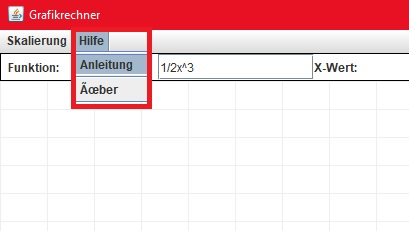
\includegraphics[width=0.4\textwidth]{Bilder/GR_7.jpg} }
	\hspace{1cm}
		\subfloat[Extrafenster für die Anleitung]{
		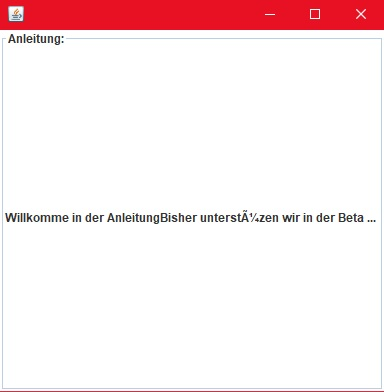
\includegraphics[width=0.4\textwidth]{Bilder/GR_8.jpg} }
	\end{center}
\end{figure}


%-----------------------------------------------------------------------------------------





